\lab{Trust-Region Methods}{Trust-Region Methods}
\label{lab:trust_region}

\objective{Explore Trust-Region methods for optimization.}

When it comes to optimizing high-dimensional functions, a common strategy is to break
the problem up into a series of smaller, easier tasks, leading to a sequence of
successive approximations to the optimizer. This is the approach taken by Line-Search
algorithms such as Newton's method or conjugate gradient.
The class of algorithms known as trust-region methods are also based on this
strategy, although they differ from line-search methods in some important ways.

\section*{Overview of the Trust-Region Approach}
Suppose we wish to minimize a function $f$.
Given some particular point $x_k$ in the domain of $f$, how do we
select a new point $x_{k+1}$ that better minimizes the function? A line-search
algorithm solves this sub-problem by first choosing a search direction $d_k$
(often related to the gradient of $f$), and then a step length $\alpha_k$ so
as to minimize $f$ along the direction $d_k$. The next point, then, is simply
\[
x_{k+1} := x_k + \alpha_k d_k.
\]

A trust-region algorithm, on the other hand, does away with a search direction and
step length, and instead approximates the function $f$ with some simpler function
$m_k$ (called the \emph{model function}) in a neighborhood of $x_k$.
The model $m_k$ will likely not be a good approximation for $f$ over the entire
domain, and so we must restrict our attention to a ball of radius $r_k$ centered at
the point $x_k$, inside of which $m_k$ is reasonably close to $f$. We then minimize
$m_k$ over this ball, and set $x_{k+1}$ equal to this minimizer. That is, we compute $x_{k+1}$ by
solving the sub-problem
\[
x_{k+1} := \underset{x \in B(x_k, r_k)}{\text{argmin}} m_k(x).
\]
The ball $B(x_k, r_k)$ is called the \emph{trust region} because we trust that the
model function $m_k$ gives a reasonably accurate approximation of $f$ on this region.
Note that it is also possible to use other types of trust regions, such as
ellipsoidal or box-like regions.

\subsection*{The Model Function}
The model function is commonly taken to be a linear or quadratic approximation of
$f$ based on its Taylor Series expansion about the point $x_k$. In the linear case,
our model function has the form
\[
m_k(x) = f(x_k) + (x-x_k)^T \nabla f(x_k).
\]
In the quadratic case, we simply add on a quadratic term to obtain
\[
m_k(x) = f(x_k) + (x-x_k)^T \nabla f(x_k) + \frac{1}{2}(x - x_k)^T H_k (x-x_k),
\]
where $H_k$ is the Hessian matrix of $f$ at $x_k$, or some approximation thereof.
Given a trust region with radius $r_k$, note that our sub-problem can be
written in the following way:
\begin{align*}
x_{k+1} &= \underset{x \in B(x_k, r_k)}{\text{argmin}} m_k(x)\\
&= x_k + p_k,
\end{align*}
where
\begin{equation}
p_k = \underset{\|p\| < r_k}{\text{argmin}}\, \{f(x_k) + p^T \nabla f(x_k) + \frac{1}{2}p^T H_k p\}.
\label{eq:step}
\end{equation}
$p_k$ is called a \emph{step}.
Also we define $p$ to be
\begin{equation}
p = x - x_k
\end{equation}

For the remainder of the lab, we define
\[
m_k(p) = f(x_k) + p^T \nabla f(x_k) + \frac{1}{2}p^T H_k p,
\]
and refer to \emph{this} function as the model function.

\subsection*{The Trust-Region Radius}
A crucial aspect of trust-region algorithms is the choice of radius $r_k$. If $r_k$ is too small, then the algorithm will
make slow progress toward the minimizer of $f$. If $r_k$ is too large, the model function will be a poor fit for the objective
function $f$, and the next iterate $x_{k+1}$ may fail to decrease $f$.
Of course, whether the radius is too small or large depends on the local behavior of $f$, which may change as the algorithm
converges. A reasonably robust trust-region algorithm must therefore be able to adaptively choose the trust-region radius.

Our strategy for choosing an appropriate radius $r_{k+1}$ for the $(k+1)$-th iterate involves evaluating the accuracy
of the model function at the $k$-th iterate. If the model was accurate and a large step was taken, we can optimistically choose $r_{k+1}$ to be larger
than $r_k$ in the hopes of achieving faster convergence.
To prevent the radius from growing too large, we set an overall bound $r_{max}$ on the trust-region radii.
If the model was very inaccurate, we make $r_{k+1}$ smaller than
$r_k$, since the model function can't be trusted over such a large region. If the model was neither particularly accurate
nor inaccurate, we simply choose $r_{k+1} = r_k$.

We measure the accuracy of the model by computing the following value:
\[
\rho_k = \frac{f(x_k)-f(x_k+p_k)}{m_k(0) - m_k(p_k)}.
\]
This value is the ratio of the \emph{actual reduction} to the \emph{predicted reduction} in the objective function. The closer
$\rho_k$ is to $1$, the more accurate the model.
Note that if $\rho_k$ is negative or below a certain positive threshold $\eta$,
then the point $x_k+p_k$ is a poor improvement over $x_k$ (and perhaps is worse).
In this case, we reject the new point and set $x_{k+1} = x_k$.

\subsection*{The Trust-Region Algorithm}
We now combine the two steps of minimizing the model function and choosing the trust-region radius to build the algorithm.  In practice, we halt the algorithm once $\|\nabla f(x_k)\|$ is less than some threshold value.
\begin{algorithm}
\begin{algorithmic}[1]
\Procedure{Trust-Region Algorithm}{}
    \State Choose initial point $x_0$, initial radius $r_0$, and threshold $\eta \in [0,0.25)$.
    \While{$\|\nabla f(x_k)\|>tol$}
        \State Calculate $p_k$ by solving the sub-problem in Equation \ref{eq:step}.
        \State Compute $\rho_k$.
        \If{$\rho_k < 0.25$}
            \State $r_{k+1} = 0.25r_k$

        \Else
            \If{$\rho_k > 0.75$ and $\|p_k\| = r_k$}
                \State $r_{k+1} = \min(2r_k, r_{max})$
            \Else
                \State $r_{k+1} = r_k$
            \EndIf
        \EndIf
        \If{$\rho_k > \eta$}
            \State $x_{k+1} = x_k + p_k$
        \Else
            \State $x_{k+1} = x_k$
        \EndIf
    \EndWhile
\EndProcedure
\end{algorithmic}
\caption{Trust-Region Algorithm}
\label{alg:trustregion}
\end{algorithm}

\begin{problem}
Implement the trust-region algorithm using the following function declaration.  Note that you don't have to actually solve (\ref{eq:step}) for $p_k$; you'll worry about that in Problem \ref{prob:dogleg}. In the mean time, you have a parameter \li{subprob} which you can assume does that for you. The function \li{subprob()} takes as parameters a gradient vector, hessian matrix, and radius.
\begin{lstlisting}
def trustRegion(f,grad,hess,subprob,x0,r0,rmax,eta=1./16,gtol=1e-5):
    """
    Minimize a function using the trust-region algorithm.

    Parameters
    ----------
    f : callable function object
        The objective function to minimize
    g : callable function object
        The gradient (or approximate gradient) of the objective function
    hess : callable function object
        The hessian (or approximate hessian) of the objective function
    subprob: callable function object
        Returns the step p_k
    x0 : numpy array of shape (n,)
        The initial point
    r0 : float
        The initial trust-region radius
    rmax : float
        The max value for trust-region radii
    eta : float in [0,0.25)
        Acceptance threshold
    gtol : float
        Convergence threshold

    Returns
    -------
    x : the minimizer of f

    Notes
    -----
    The functions f, g, and hess should all take a single parameter.
    The function subprob takes as parameters a gradient vector, hessian matrix, and radius.
    """
    pass
\end{lstlisting}
\end{problem}

\subsection*{Solving the Sub-problem: the Dogleg Method}
Our trust-region algorithm is as yet incomplete, since we do not have a viable means solving the subproblem
given by Equation \ref{eq:step}.
We may be tempted to search for the true minimizer of the model function over the trust region, but it turns out
that we can get away with just an approximate minimizer.
We will employ the ``dogleg" method when selecting an approximate minimizer of the model function.
This method works by minimizing the model function along a particular path extending from the origin out
to the boundary of the trust region.
This path is piecewise linear and has a shape vaguely reminiscent of a dog's leg, which explains the peculiar name of the method.

To calculate the dogleg minimizer of the model function, we first solve the unconstrained minimizer of the model function.  We $p^B$ as the unconstrained minimizer of the model function:
\[
p^B = -H_k^{-1}\nabla f(x_k).
\]
We then calculate the direction of steepest descent for the model function, given by
\[
p^U = -\frac{\nabla f(x_k)^T\nabla f(x_k)}{\nabla f(x_k)^TH_k\nabla f(x_k)}\nabla f(x_k).
\]
We define the dogleg path using these two points as follows:
\[
\gamma(\tau) =  \left\{
     \begin{array}{lr}
       \tau p^U, & 0\leq \tau \leq 1\\
       p^U+(\tau-1)(p^B-p^U), & 1\leq \tau\leq 2
     \end{array}
   \right.
\]

\begin{figure}
\centering
    \begin{subfigure}[b]{0.3\textwidth}
            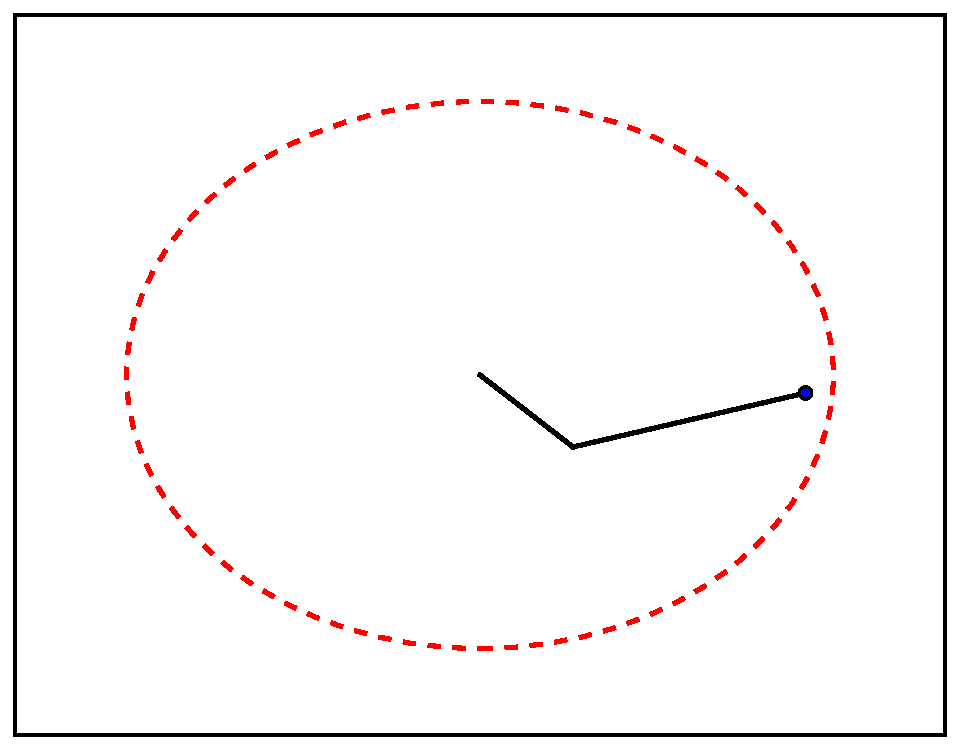
\includegraphics[width=\textwidth]{dogleg3}
            \caption{Dogleg path completely within the trust region.}
            \label{fig:dl3}
    \end{subfigure}%
    ~ %add desired spacing between images, e. g. ~, \quad, \qquad, \hfill etc.
      %(or a blank line to force the subfigure onto a new line)
    \begin{subfigure}[b]{0.3\textwidth}
            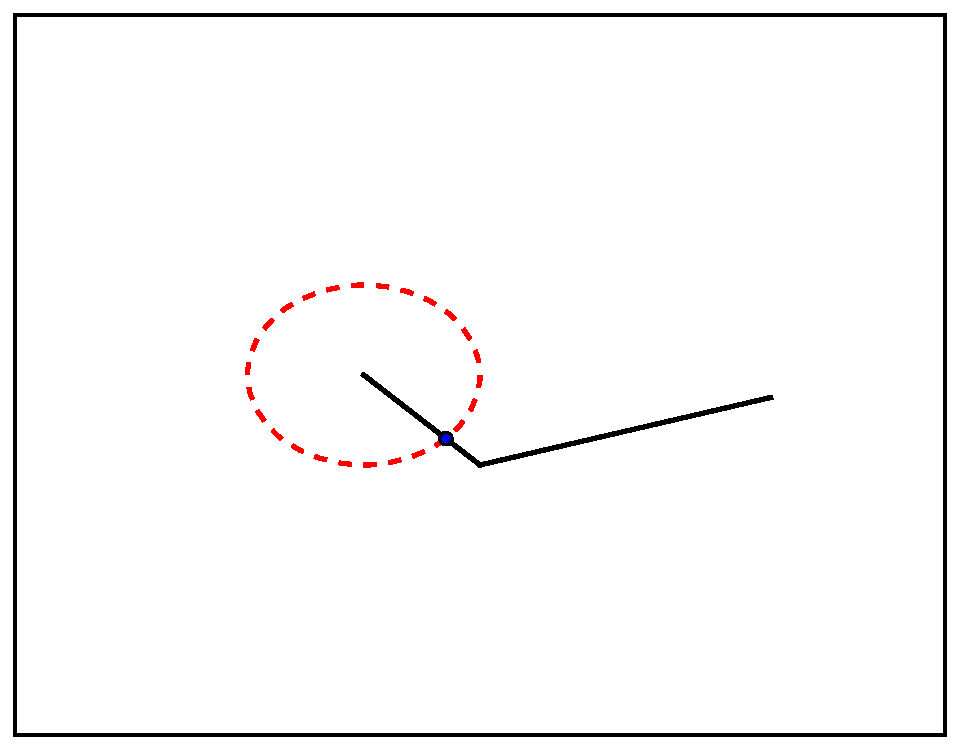
\includegraphics[width=\textwidth]{dogleg1}
            \caption{Intersection in the first leg of the path.}
            \label{fig:dl1}
    \end{subfigure}
    ~ %add desired spacing between images, e. g. ~, \quad, \qquad, \hfill etc.
      %(or a blank line to force the subfigure onto a new line)
    \begin{subfigure}[b]{0.3\textwidth}
            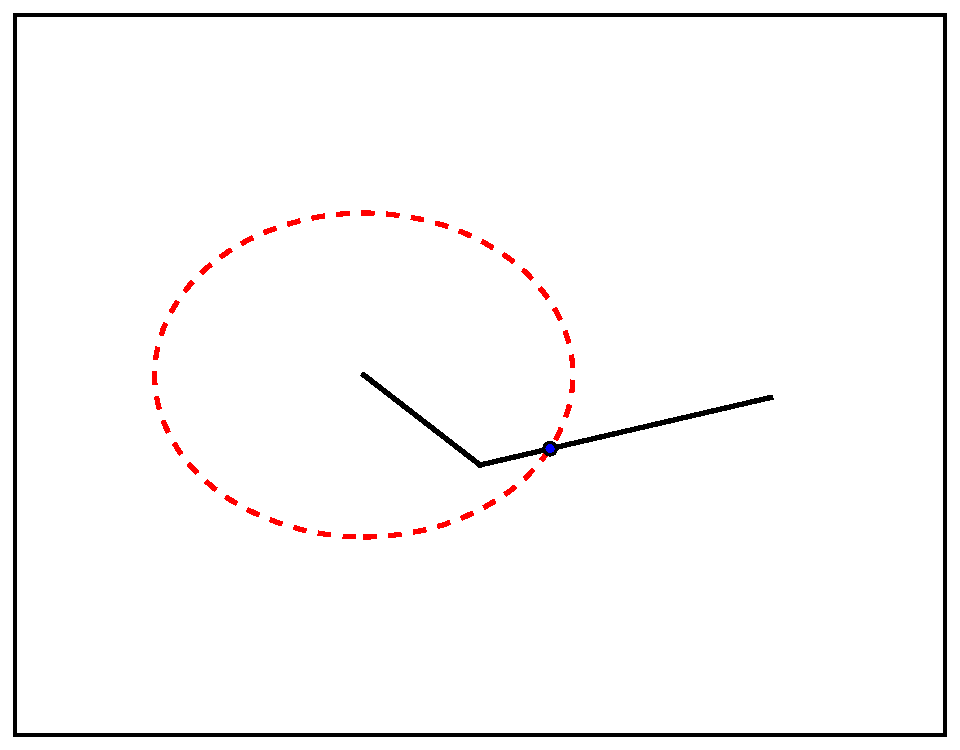
\includegraphics[width=\textwidth]{dogleg2}
            \caption{Intersection in the second leg of the path.}
            \label{fig:dl2}
    \end{subfigure}
    \caption{Relationships between the dogleg path (black solid line),
    the trust region boundary (red dashed circle), and the dogleg minimizer (blue dot).}
    \label{fig:dogleg}
\end{figure}

It can be shown that the model function decreases along this path. Thus,
the dogleg minimizer is either the endpoint of the path if it lies completely within the trust region,
or the point of intersection between the path and the boundary of the trust region.
See Figure \ref{fig:dogleg} for an illustration of the three salient cases. We consider each case in turn.
\begin{itemize}
\item
When the path lies completely within the trust region, the dogleg minimizer is simply the endpoint, namely $p^B$.
This is the case when $\|p^B\| \leq r_k$. See Figure \ref{fig:dl3}.
\item
When the path intersects the boundary of the trust region in the first line segment, the dogleg minimizer is
$r_kp^U/\|p^U\|$.
This is the case when $\|p^U\| \geq r_k$. See Figure \ref{fig:dl1}.
\item
When the path intersects the boundary of the trust region in the second line segment, the dogleg minimizer is
given by $p^U + (\tau^*-1)(p^B-p^U)$, where $\tau^*$ satisfies the quadratic equation
\[
\|p^U + (\tau^*-1)(p^B-p^U)\|^2 = r_k^2.
\]
This quadratic equation can be simplified into 
\[
a(\tau^*-1)^2+b(\tau^*-1)+c = 0
\]
where the coefficients are defined to be
\[
a = p_B^Tp_B - 2p_B^Tp_U+p_U^Tp_U
\]
\[
b = 2p_B^Tp_U-2p_U^Tp_U
\]
\[
c = p_U^Tp_U-r_k^2.
\]
See Figure \ref{fig:dl2}.
\end{itemize}

\begin{problem}
Implement the dogleg method using the following function declaration.
Remember to avoid calculating the inverse of a matrix.
\begin{lstlisting}
def dogleg(gk,Bk,rk):
    """
    Calculate the dogleg minimizer of the quadratic model function.

    Parameters
    ----------
    gk : ndarray of shape (n,)
        The current gradient of the objective function
    Bk : ndarray of shape (n,n)
        The current (or approximate) hessian
    rk : float
        The current trust region radius

    Returns
    -------
    pk : ndarray of shape (n,)
        The dogleg minimizer of the model function.
    """
    pass
\end{lstlisting}

\label{prob:dogleg}
\end{problem}

Test your implementation of the trust-region algorithm on the Rosenbrock function contained the {\tt scipy.optimize} module.
Compare your answer with that obtained by SciPy's trust-region implementation. The code to accomplish this, together with the
correct results, is given below.
\begin{lstlisting}
>>> from scipy import optimize as op
>>> x = np.array([10.,10])
>>> rmax=2.
>>> r=.25
>>> eta=1./16
>>> tol=1e-5
>>> opts = {'initial_trust_radius':r, 'max_trust_radius':rmax, 'eta':eta, 'gtol':tol}
>>> sol1 = op.minimize(op.rosen, x, method='dogleg', jac=op.rosen_der, hess=op.rosen_hess, options=opts)
>>> sol2 = trustRegion(op.rosen, op.rosen_der, op.rosen_hess, dogleg, x, r, rmax, eta, gtol=tol)
>>> print np.allclose(sol1.x, sol2)
True
\end{lstlisting}
\begin{problem}
Test your \li{trustRegion()} and \li{dogleg()} methods on the Rosenbrock function.  Use the \li{rosen()}, \li{rosen_der()}, and \li{rosen_hess()} methods from \li{scipy.optimize}.  Return the solution \li{x*} from the \li{trustRegion()} method.
\end{problem}

\subsection*{Solving Systems of Nonlinear Equations}
Trust-region methods can be used to find solutions of systems of nonlinear equations, which arise in applications across science and engineering.
Suppose we have a vector function $r : \mathbb{R}^n \rightarrow \mathbb{R}^n$, written as
\[
r(x) = \begin{bmatrix}
r_1(x)\\
r_2(x)\\
\vdots\\
r_n(x)
\end{bmatrix},
\]
where each $r_i$ is a nonlinear smooth function mapping from $\mathbb{R}^n$ into $\mathbb{R}$.
Our goal is to find $x \in \mathbb{R}^n$ that satisfies $r(x) = 0$; such an $x$ is called a solution
or root of the nonlinear system. In general, there may be several roots (even infinitely many), or there
may be none at all. Solving the equations by hand can range from arduous to impossible, so we turn
to trust-region methods for help.

In order to use our trust-region method to find the roots of a system
of equations, we need to come up with an objective function whose minima correspond to roots of the
system. As such, we consider the \emph{merit function}
\[
f(x) = \frac{1}{2}\|r(x)\|_2^2 = \frac{1}{2}\sum_{i=1}^nr_i(x)^2,
\]
which, roughly speaking, measures how close a point $x$ is to being a root of $r$. Note that $f(x) = 0$
if and only if $r(x) = 0$. Thus, if we can successfully find a global minimum of $f$, we will have
found a root to the nonlinear system.

Now that we have an objective function, we need to create a quadratic model function. If we let
$J_k$ be the Jacobian matrix of $r$ at the point $x_k$, i.e.
\[
J_k = \begin{bmatrix}
\nabla r_1(x_k)^T\\
\nabla r_2(x_k)^T\\
\vdots\\
\nabla r_n(x_k)^T
\end{bmatrix},
\]
then we can write the gradient $\nabla f(x_k) = J_k^Tr(x_k)$ and the Hessian $H_k = J_k^TJ_k$.
We can now use the same model function described earlier.

Let's work through an example. Consider the system
\[
r(x,y) = \begin{bmatrix}
-\sin x\cos y - 2\cos x\sin y\\
-\sin y\cos x - 2\cos y\sin x
\end{bmatrix}.
\]
Observe that the Jacobian takes the form
\[
J(x) = \begin{bmatrix}
-\cos x\cos y + 2\sin x\sin y & \sin x\sin y - 2\cos x\cos y\\
\sin y\sin x - 2\cos y\cos x & -\cos y\cos x + 2\sin y \sin x
\end{bmatrix}.
\]
In Python, we initialize all of the requisite functions and then find a root as follows:
\begin{lstlisting}
>>> # define the system of equations
>>> def r(x):
>>>     return np.array([-sin(x[0])*cos(x[1]) - 2*cos(x[0])*sin(x[1]),
>>>                      -sin(x[1])*cos(x[0]) - 2*cos(x[1])*sin(x[0])])
>>>
>>> # define the merit function
>>> def f(x):
>>>     return .5*(r(x)**2).sum()
>>>
>>> # define the jacobian function
>>> def J(x):
>>>     return np.array([[-cos(x[0])*cos(x[1]) + 2*sin(x[0])*sin(x[1]),
>>>                       sin(x[0])*sin(x[1]) - 2*cos(x[0])*cos(x[1])],
>>>                      [sin(x[1])*sin(x[0]) - 2*cos(x[1])*cos(x[0]),
>>>                       -cos(x[1])*cos(x[0]) + 2*sin(x[1])*sin(x[0])]])
>>>
>>> # define the gradient function
>>> def g(x):
>>>     return J(x).dot(r(x))
>>>
>>> # define the Hessian function
>>> def H(x):
>>>     return J(x).T.dot(J(x))
>>>
>>> # set trust-region parameters
>>> rmax=2.
>>> rr=.25
>>> eta=1./16
>>> tol=1e-5
>>> # set initial point
>>> x = np.array([3.5, -2.5])
>>> # find a minimizer of f
>>> xstar = trustRegion(f,g,H,dogleg,x,rr,rmax,eta=eta,gtol=tol)
>>> print xstar
[ 3.14159265 -3.14159265]
>>> # verify that it is a root of r
>>> print r(xstar)
[ -7.75116117e-09   7.75147025e-09]
\end{lstlisting}

Of course, we are not guaranteed to always find a root, as convergence depends on the choice of initial point.
However, by running the algorithms with several randomly selected starting points, we are more likely to 
be successful.
\begin{problem}
Solve the following system
\[
r(x,y) = \begin{bmatrix}
\sin x\cos y - 4\cos x\sin y\\
\sin y\cos x - 4\cos y\sin x
\end{bmatrix} 
= \begin{bmatrix}
0\\
0
\end{bmatrix}.
\]
\end{problem}

\begin{comment}
\begin{problem}
Some problem involving system of nonlinear equations. Consult http://www-sop.inria.fr/coprin/logiciels/ALIAS/Benches/ 
for ideas.
\end{problem}
\end{comment}
